\documentclass{article}
%Nu tester jeg lige igen
% Language setting
% Replace `english' with e.g. `spanish' to change the document language
\usepackage[danish]{babel}
% Set page size and margins
% Replace `letterpaper' with `a4paper' for UK/EU standard size
\usepackage[a4paper,top=2cm,bottom=2cm,left=3cm,right=3cm,marginparwidth=1.75cm]{geometry}

% Useful packages
\usepackage{amsmath}
\usepackage{graphicx}
\usepackage[colorlinks=true, allcolors=blue]{hyperref}
\usepackage{array}

\title{CDIO delopgave 1}
\author{Jakob Agergaard}


\begin{document}




\begin{titlepage}
\begin{center}

    
\includegraphics[width=0.25\textwidth]{Billeder/DTULogo.png} \\
    \vspace{0.5cm}
    \Large
    \textbf{02314\hspace{1cm}62531\hspace{1cm}62532} \\
    Indledende programmering, Udviklingsmetoder til IT-systemer og Versionsstyring og testmetoder
    \vspace{0.4cm}
    \hrule
    
    \vspace*{0.5cm}
    \huge
    \textbf{CDIO delopgave 1}\\
    \LARGE
    Gruppe 17
    \vspace{0.5cm}
    \hrule
    \vspace{0.2cm}

    \large
    \begin{tabular}{m{10em} m{8em} m{8em} m{10em}}
    Jakob Skov Agergaard\vfill s224570 & 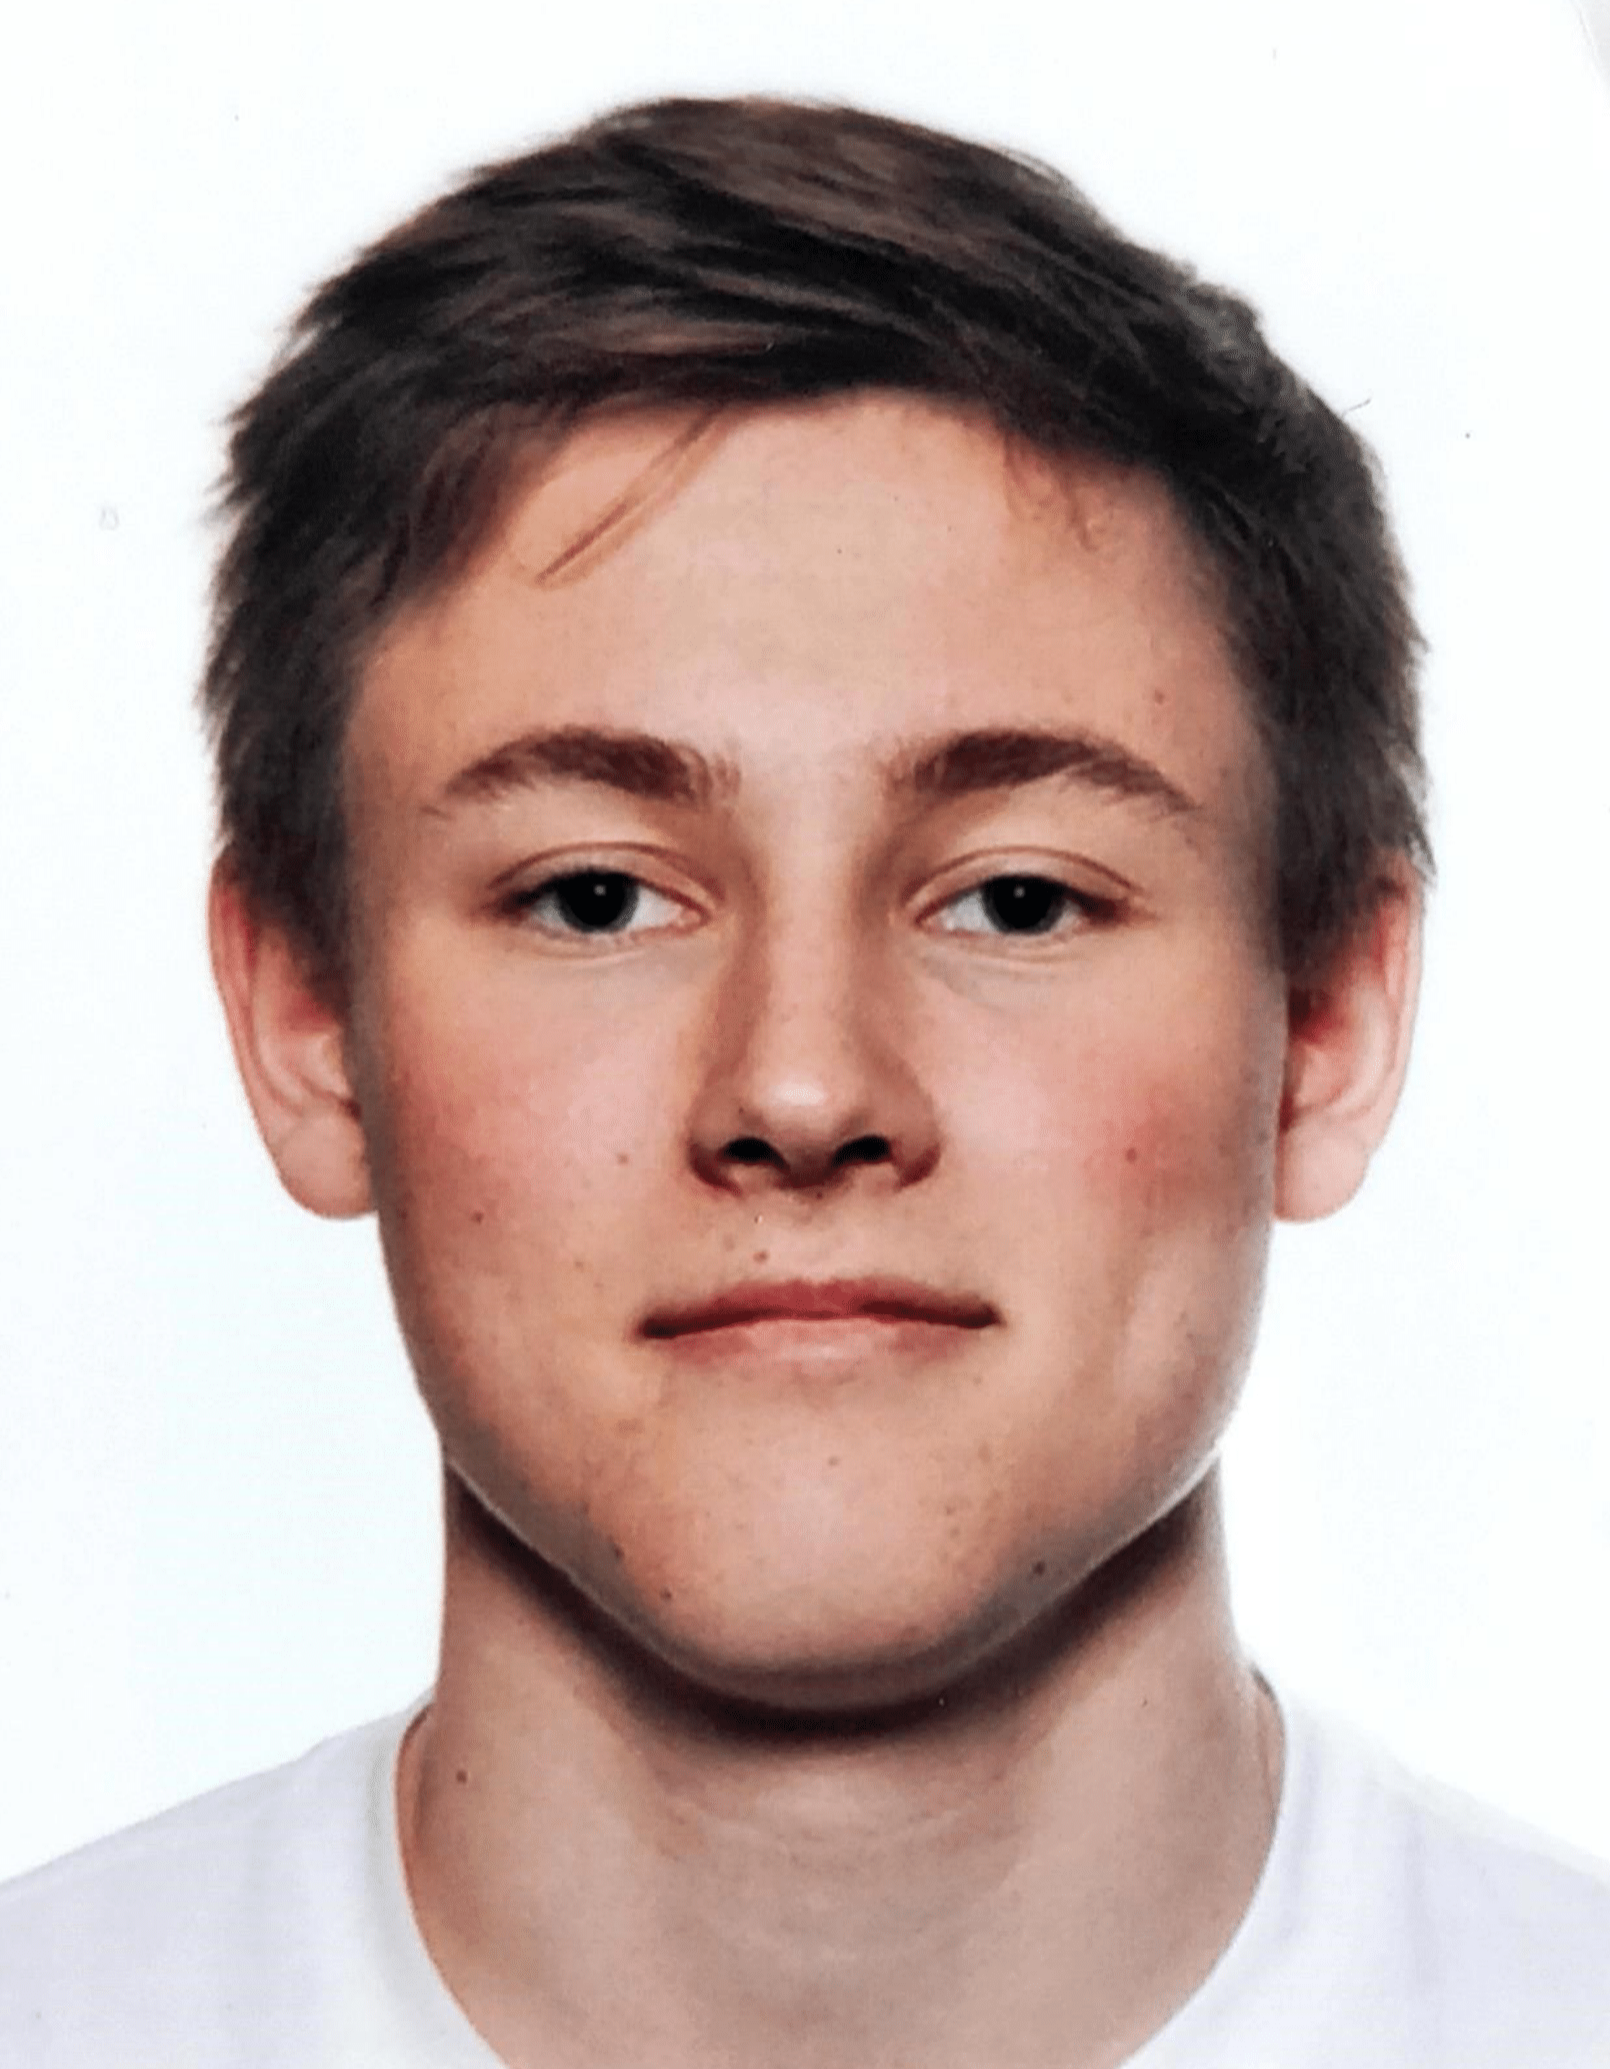
\includegraphics[width=0.2\textwidth]{Billeder/JakobFoto.png} & 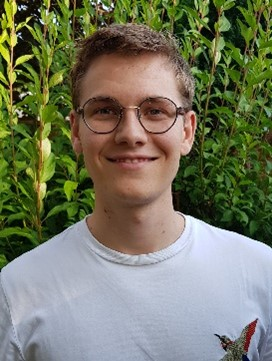
\includegraphics[width=0.2\textwidth]{Billeder/PhilipFoto.jpg} & Philip Muff Førrisdahl\vfill s224566 \\
    Mads Fogelberg Hansen\vfill s224563 & 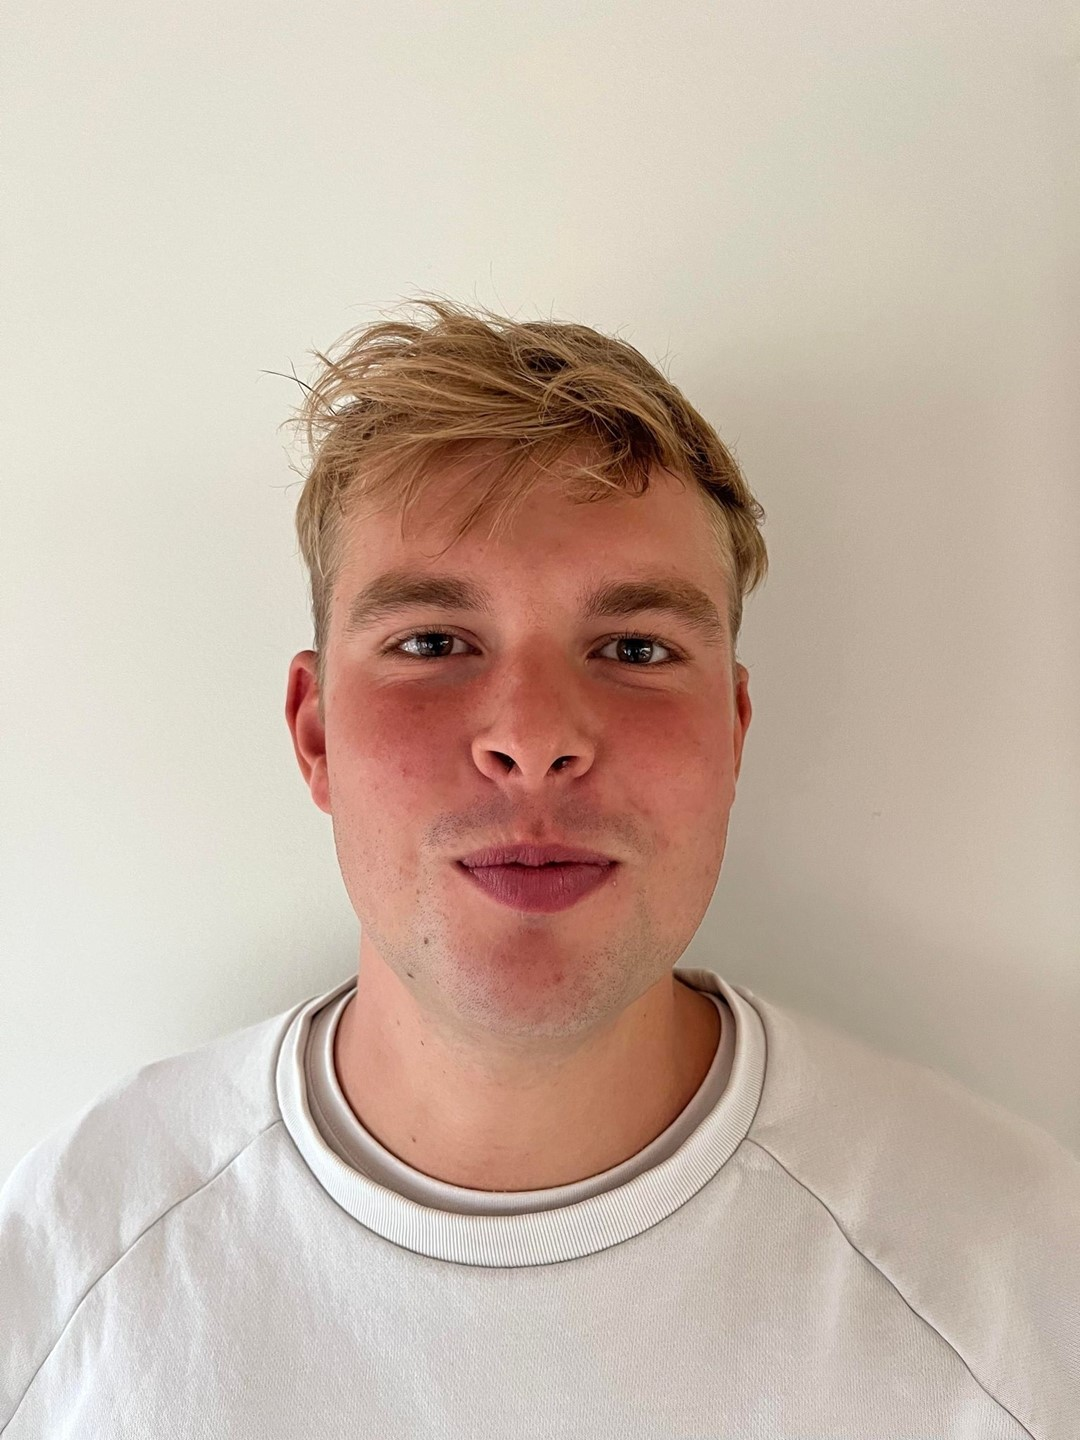
\includegraphics[width=0.2\textwidth]{Billeder/FotoMads.jpg} & 
\includegraphics[width=0.2\textwidth]{Billeder/EsbenFoto.png} & Esben Skovmand Elnegaard \vfill s224555  \\
    Jarl Boyd Roest\vfill s224556 & 
\includegraphics[width=0.2\textwidth]{Billeder/JarlFoto.png}
    \end{tabular}

    \vfill
    
    
    \vspace{1cm}
    \LARGE
    18. september 2022

    \vspace{1cm}
    
\end{center}
\end{titlepage}


\normalsize
\begin{abstract}
     Her kommer der et resume af opgaven
\end{abstract}

\tableofcontents

\section{Timeregnskab}
Hej her kommer timeregnskabet det er work in progress

\section{Indledning}

Her kommer indledningen...
Godmoorgen

\section{Projekt-planlægning}
\begen {itemize}
\item Vi strukturerede, ummidelbart efter feedback fra projektlederen, en plan for udviklingen af projektet og programmet jf. kravspecifikationerne. Vi så på opgaverne og kravene til spillet, der var var slået på plads dag 1, og prioriterede opgaverne som følgende
 \item Uge 1:
 Opgaver:
Prioirteret. (19-09-2022) udkast.
Versionsstyringen af programmet samt dokumentation for alle gruppemedlemmer
Use case(s), evt. diagrammer
Random nr generator samt test + terningkast og test.
Interface relaterede funktioner (navn, pointtæller, turskift, antal ture)
\item Uge 2:
Opdaterede opgaver (26-09-2022)
Opgaver løst:
Versionering af programmet
Diagram (sekvens)
test af terninger
nterface kode: navn, pointtæller, turskift, antal ture

\item Nye opgaver:
Prioriteret
Færdigudiviklen koden uden redepmtionfaktor
Opdatering af sekvens diagram samt klassediagram
Rapportere udvikling i rapporten.
Sekundære funktioner skal implementeres (coinflip)

 
\section{Krav/Analyse}
For at have en mere præcis kravsspecifikation startede vi med at spørge vores projektleder om følgende spørgsmål:
\begin{itemize}
    \item [Q:] hvilken version af Java har maskinerne installeret?
            \subitem A: Den nyeste version (18).
    \item [Q:]Hvilke input-metoder er tilgængelig?
            \subitem A: Både mus og tastatur.
    \item [Q:]Skal de 2 spillere have samme input-metode?
            \subitem A: De skal ikke, men kan godt.
    \item [Q:]Skal pointene være synlige for alle spillere eller blot nogle?
            \subitem A: Ja, synlige for alle.
    \item [Q:]Kan spillerne ende med mere end 40 point?
            \subitem A: Ja
    \item [Q:]Er vinderen den der når 40 point først? Hvad hvis de rammer 40 point på samme tur?
            \subitem A: Det er antallet af ture der tæller. Hvis begge spillere får 40 eller over, i samme tur spiller, er vinderen den der slår højest i næste slag. Hvis lige fortsættes dette.
    \item [Q:]Hvad er et almindeligt menneske?
            \subitem A: Alle der besidder over 8. klasse pc færdighed, er op til 80 år gamle og har et almindeligt helbred.
    \item [Q:] Skal spillerne have navne?
            \subitem A: Ja
    \item [Q:]Hvem skal starte?
            \subitem A: Dette bestemmes ved et "coin flip". Altså helt tilfældigt.
    \item [Q:]Hvad er formålet med testen. Hvad ønskes der testet udover systemet funktionalitet som helhed?
        \subitem A: At de virtuelle terninger, statistisk opfører sig som normale terninger.
\end{itemize}

\section{Design}


\section{Implementering}

\section{Test}
Der er blevet bedt om en test af de to terninger, som indgår i vores terningespil. Hensigten ved at teste terningerne er at se p ̊a sandsynligheden for de forskellige udfald. De forskellige udfald skal stemmer overens med normalfordelingen af to terninger. En normal fordeling er karakteriserede ved at have en ”klokke”formede kurve. 

Der vil automatisk være kast, som er hyppigere end andre, da der er flere kombinationer som giver det samme. Det vil for eksempel være tallene 5, 6 og 7, som vil være de mest hyppige kast, fordi der er flest forskellige kombinationer som kan slå disse tal. Normal fordelingen for 2 terninger kan ses p ̊a figur 7.1


Billede af normalfordelingen af to terninger


Vores test af terningerne er lavet i Intellij, som tager udgangspunkt i i de to terninger, som skal indgå i terningespillet. Terninger er blevet slået 10.000 gange for at få et mere præcis resultat. Man kan få et endnu mere præcis resultat, hvis man lavede flere terningkast, da det vil give flere observationer, og dermed en bedre normalfordeling.
Testen af vores 2 terninger kan se i følgende figur 7.2

- billede af test


Ved at sammenligne figur 7.1 og 7.2, kan man hurtigt se at de som udgangs er meget ens. Begge figurer har en "klokke" formede kurve, som var det målet var. Der er nogle små ud svingninger i vores kurve, hvilket vil kunne løses ved at lave flere kast, som vil gøre det mere præcist 


\section{Konklusion}

\section{Bilag}
\subsection{Litteratur}
\subsection{Kode}

\end{document}